\documentclass[12pt,a4paper]{article}

\usepackage{todonotes}
\usepackage{float}
\usepackage{pdflscape}
\usepackage{parskip}
\usepackage[hyphens]{url}
\usepackage[hidelinks]{hyperref}
\usepackage[margin=3.5cm]{geometry}
\usepackage{graphicx}
\usepackage[bottom]{footmisc}

%%%%%%%%%%%%%%%%%%%%%%%%%%%%%%%%%%%%%%%%%%%%%%%%%%%%%%%%%%%%%%%%%%%%%%%%%%%%%%%%
% BIBLATEX SETTINGS
%%%%%%%%%%%%%%%%%%%%%%%%%%%%%%%%%%%%%%%%%%%%%%%%%%%%%%%%%%%%%%%%%%%%%%%%%%%%%%%%
\usepackage[
backend=bibtex,
firstinits=true,    % Render first and middle names as initials
maxcitenames=2,     % Use maximum 2 names in \cite before et al.
maxbibnames=99,      % Use maximum 2 names in references before et al.
style=authoryear,
dashed=false,       % Re-print recurring author names in bibliography
]{biblatex}

% Use single quotes around titles:
\usepackage[british]{babel}
\usepackage{csquotes}

% Add a blank line between references
\setlength{\bibitemsep}{\baselineskip}

% Don't use reference months
\AtEveryBibitem{\clearfield{month}}
\AtEveryCitekey{\clearfield{month}}

% All author's names should be Last, First
\DeclareNameAlias{author}{last-first}

% Insert a comma between author and year in text citations
\renewcommand*{\nameyeardelim}{\addcomma\addspace}

% Remove 'in:' preceding article title
\renewbibmacro{in:}{}

\addbibresource{../bibliography.bib}

%%%%%%%%%%%%%%%%%%%%%%%%%%%%%%%%%%%%%%%%%%%%%%%%%%%%%%%%%%%%%%%%%%%%%%%%%%%%%%%%

\begin{document}
\listoftodos[Todo]
\pagebreak

\begin{titlepage}
\center
\vspace*{3cm}

{\Large
    Electronics and Computer Science\\
    Faculty of Physical Sciences and Engineering\\
    University of Southampton\\[1cm]
}

Jamie Davies\\
%\href{mailto:jagd1g11@ecs.soton.ac.uk}{\nolinkurl{jagd1g11@ecs.soton.ac.uk}}\\[3cm]
\today\\[1cm]

{\large
    Enhanced Content Analysis and Information\\
    Retrieval Using Twitter Hashtags\\[1cm]
}

A project report submitted for the award of\\
MEng Computer Science\\[1cm]

\emph{Supervisor:}\\
Dr. Nick Gibbins\\[0.5cm]
%\href{mailto:nmg@ecs.soton.ac.uk}{\nolinkurl{nmg@ecs.soton.ac.uk}}\\[0.5cm]

\emph{Examiner:}\\
Dr. Klaus-Peter Zauner\\
%\href{mailto:kpz@ecs.soton.ac.uk}{\nolinkurl{kpz@ecs.soton.ac.uk}}\\


\vfill
\end{titlepage}

\section*{Abstract}
One of the key characteristics of Twitter and other microblogging platforms is the use of `hashtags' --- topical/categorical annotations provided by the authors of the posts (tweets) themselves. This flexible system was designed for the effective organisation and searching of tweets, but with Twitter facing an ever-increasing number of users and tweets it is hard for users to keep track of the vast number of hashtags in popular use. This results in data from the hashtags being fragmented and inaccurate due to the users making poor or uninformed hashtag choices.

If users are presented with a choice of relevant hashtags when writing a tweet, they are more likely to publish tweets with accurate tag data. This project aims to create an intelligent hashtag recommendation tool to raise the information gain from hashtags. However, whilst such a system could improve the quality of the hashtag data for future tweets, tweets that have already been published will remain untouched by the system. Thus, the system will be extended to also retrofit hashtags to published tweets --- allowing for tweets to appear in search results for a particular hashtag even if they don't actually contain the hashtag in question.
\pagebreak

\tableofcontents

\pagebreak

\section{Introduction}
Collaborative tagging (sometimes referred to as social tagging) systems are designed to allow users to navigate, organise and manage online resources. The central idea behind these systems is the concept of an annotation: the action of a user applying a personalised tag to a resource. On a large scale, many of these annotations can be taken together to form a complex network of users, resources and tags --- commonly referred to as a \emph{folksonomy} \parencite{Xu:2008}.

One of the most popular applications of a folksonomy is Twitter\footnote{\url{www.twitter.com}}. `Hashtags,' which are simply any combination of letters or digits preceded by a hash character (\#), afford users the ability to create free-form tags to describe the content of their posts (tweets). Tweets can be categorized with several hashtags, thereby creating networks of tweets and users and making it easy to find other related tweets, users and hashtags. This renders hashtags as a powerful tool in aiding the search and navigation of the billions of tweets contained within Twitter.

Despite its numerous benefits, the hashtag system presents new challenges to overcome before they can become truly useful. Due to the open nature of folksonomies, it is important that users have the freedom to create and use exactly the tags they wish to use. However, this unsupervised tagging can result in vast numbers of hashtags for users to choose from --- often including redundant or ambiguous hashtags. When posting a tweet, there is nothing stopping a user from creating an entirely new hashtag to describe something with exactly the same meaning as a collection of other hashtags. This tag redundancy confuse users and fragment the true meaning behind the synonymous hashtags.

\subsection{Project Goals}
\label{sec:goals}
This project will create a system that aims to support and enrich the information provided by hashtags on Twitter. It will use a combination of different machine-learning techniques to examine and classify the topics and concepts behind the hashtags and in doing so, be able to suggest suitable hashtags for tweets that are relevant to their content. This will allow users to make a better choice of hashtag when writing tweets, and therefore refine the information that they provide.

However, as suggesting better hashtags will only improve the information gain from future tweets, the system will be extended to provide a context-aware tweet search facility. This will enable users to search for a particular hashtag, and instead of only returning tweets containing that hashtag (as current systems do), it will also provide tweets that are contextually relevant to the search term but do not contain that given hashtag.

Through the creation of the system, new insights and understanding of how people use Twitter could come to light. This provides the possibility to attempt to answer optional interesting questions, such as
\begin{itemize}
    \item Are certain types of tweet/hashtag easier to classify than others?
    \item Is it possible to make relevant hashtag suggestions using just the tweet text itself, or is other metadata needed to make the recommendations useful?
\end{itemize}

\pagebreak

\section{Background and Literature Review}
\label{sec:litreview}
The main design goals behind hashtags are to categorise tweets and allow them to show up more easily in searches\footnote{\url{https://support.twitter.com/articles/49309-using-hashtags-on-twitter}}. Whilst the task that this project is aiming to complete is novel and fairly unexplored, it is well connected with other experiments, systems and projects within the research community.

\subsection{Recommendation Systems}
Traditional recommendation systems are in place all over the web today. From music discovery services (such as Last.fm\footnote{\url{www.last.fm}}) to suggested purchases on retail sites (like that in place at Amazon\footnote{\url{www.amazon.co.uk}}, these systems are all personalised recommendation engines that take an individual user's preferences and use them to provide suggestions tailored to that user.

\subsubsection{Collaborative Filtering}
Most personalised recommendation systems employ a set of techniques known as collaborative filtering. These techniques were first coined by \textcite{Goldberg:1992}, where a system named \emph{Tapestry} was created that allowed people to attach annotations to documents, and then use that information to filter the documents for other users.

One common implementation of collaborative filtering is the so-called ``user-to-user'' approach. ``User-to-user'' collaborative filtering works by taking the preferences of a user $A$, and finding a small subset of other users in the system that have similar preferences. For each user $B$ in the subset any items that $B$ has adopted that $A$ hasn't are added to a ranked list of suggestions. $A$ is now more likely to adopt items in the list than the items of another random person \parencite{Schafer:2001}.

\subsubsection{Content-Based Recommendation}
Another approach to provide relevant recommendations to a user is the use of content-based recommendation systems. This is a type of system that recommends items relevant to other items by comparing the details and descriptions of the items themselves. This can be extended to suggest items for a user by comparing a content-based description of the user's preferences with the descriptions of the items \parencite{Pazzani:2007}.

A key issue with content-based filtering is that the recommendations can only be as accurate as the algorithm used to derive a user's profile. There are a number of algorithms available to build user profiles, depending upon the context, but essentially a content-based profile is created using a weighted vector of item features. The weights mark the importance of each feature to the user, and can be computed from individually rated content vectors.

\textcite{Cantador:2010} studied and evaluated a number of content-based recommendation models based upon the premise of user and item profiles being described in terms of weighted lists and tags. Through their experiments they found that models that focused on user profiles outperformed the models oriented towards item profiles in nearly every test. They go on to suggest that a better way of profiling users would be through the use of tag clustering.

\subsubsection{Relevance Feedback}
Relevance feedback is a process that was originally designed for information retrieval, and works on the assumption that a user can not always correctly encapsulate into a query what it is they are searching for. It works by allowing a user to create an initial query to which an initial set of results is returned. Out of these initial results, the user can then mark certain results as relevant or irrelevant, and this information is then submitted and used to refine the original query and return more relevant results to the user \parencite{Salton:1997}.

Instead of limiting recommendation systems to the accuracy of their classifiers, a common approach is incorporate relevance feedback techniques. \textcite{Utiyama:2006} showed that it is possible to combine collaborative filtering, content-based filtering and relevance feedback techniques into one system to provide better recommendations.

\subsection{Hashtag Recommendation Research}
Even though providing hashtag recommendations and suggestions is still a new and largely unexplored field, there have been several efforts to improve the hashtag experience for Twitter users.

\subsubsection{Current Twitter Hashtag Implementation}
The current hashtag system on Twitter (\autoref{fig:twittersuggest}) uses a non-personalised auto-complete tool to provide suggestions to the user. Whenever a hash symbol (\#) is typed in the tweet composer, the system simply suggests hashtags starting with the letters that the user has typed so far. These suggestions are chosen from a tiny subset of hashtags, taken from a mixture of the currently trending\footnote{Trending hashtags are those with the highest rise in usage within a given time period.} and from the user's history. Whilst better than not having suggestions at all, this system is only truly useful in a specific use case: when the user knows the starting letters of a trending hashtag they want to use, or are trying to recall a hashtag from they have previously used. This system does not help the user choose the correct hashtag for their tweet.

\begin{figure}
    \centering
    
\includegraphics[width=0.5\textwidth]{twittersuggest.png}
    \caption{Twitter's current hashtag suggestion system.\label{fig:twittersuggest}}
\end{figure}

\subsubsection{Comparing Tweets To Other Tweets}
By assuming that the primary purpose of hashtags is to categorise tweets and improve searching (as Twitter envisioned), \textcite{Zangerle:2011} created a system that recommends hashtags for a tweet by taking tweets from other tweets that are textually similar to the query. The similarity between tweets is calculated with the TF-IDF (term frequency -- inverse document frequency) model. The hashtags are then extracted from the similar tweets, ranked according to how similar the tweets were to the original query, and returned as a list of suggestions to the user. A number of different ranking algorithms were tested, but this was found to be the most successful.

\subsubsection{Creating Personalised Recommendations}
After studying the advantages of providing personalised recommendations in retail situations on a per-user basis, \textcite{Kywe:2012} realised that a similar approach towards hashtags could prove fruitful. Hashtag use varies from user to user, with some users using the latest trending hashtags, other uses only using a specific set or type of tag, and with some users barely using them at all. They proposed a personalised hashtag recommendation system that considers both user preferences and the query tweet content: the system creates a ranked list of hashtags from both the most similar users and most similar tweets. This gave promising results, although it was noted that this may not be the best recommendation system for all types of tweets and hashtags.

\textcite{Shepitsen:2008} used a hierarchical agglomerative clustering algorithm to profile users and provide personalised recommendations in collaborative tagging systems. They found that clusters of tags can be effectively used to ascertain a user's interests, which could then be used in a traditional content-based recommendation approach. This technique worked well, particularly for dense folksonomies such as Last.fm.

\subsubsection{Overcoming Hashtag Duality}
Observers of social media have realised that hashtags play a dual role within the online microblogging communities, such as Twitter. On one hand, hashtags fulfil the design goals that Twitter created them to accomplish (bookmarking and improving search); on the other hand, however, they serve as a badge of community membership, connecting users together. \textcite{Yang:2012} took this duality into account when attempting to create a hashtag recommendation system by training a SVM (support vector machine) classifier with a variety of features taken from the tweet metadata to overcome the duality and suggest relevant hashtags.

\subsection{Broader Classification in Twitter}
Twitter is a thriving\footnote{\url{www.bloomberg.com/news/2013-10-15/twitter-revenue-more-than-doubles-in-third-quarter.html}} metropolis of users expressing themselves on a daily (and often more frequent) basis, and has grown exponentially in size since its inception in 2006. Due to this, the data that it contains has caught the attention of researchers throughout computer science and even other disciplines. Whilst the concept of recommending hashtags is relatively unexplored, there have been many other classification experiments run with Twitter data.

\subsubsection{Categorising Tweets}
\textcite{Sriram:2010} proposed an approach to classify tweets into 5 general categories: \emph{news}, \emph{opinions}, \emph{deals}, \emph{events} and \emph{private messages}. This was achieved by using a small set of specific features from each tweet, instead of using the traditional ``Bag-Of-Words'' (BOW) text classification method. The BOW approach is centred around counting occurrences of words in the text, but in the case of Twitter and its 140 character limit, it is very rare that words are actually repeated in a tweet.

\subsubsection{Categorising Users}
Another approach to deciphering the vast quantity of data on Twitter is to classify the users themselves. Twitter has become a powerful platform for people posting content about events, and as such it would be useful to automatically establish \emph{who} is participating in these events. By taking a number of features from each user account and passing them through a K-Nearest Neighbours (KNN) algorithm, \textcite{DeChoudhury:2012} developed a system that would classify a user's behaviour into one of three categories: organisations, journalists/media bloggers and ordinary individuals.

\pagebreak

\section{Analysis \& Design}
Using knowledge gained from the background research in \autoref{sec:litreview}, the project goals described in \autoref{sec:goals} will be expanded in this section to provide an explanation of the design of the system.

\subsection{Requirements}
There are two main requirements the system in this project is aiming to fulfil. It must:
\begin{itemize}
    \item Allow users to compose and publish tweets whilst suggesting hashtags relevant to the content of their tweets.
    \item Allow users to search for a hashtag and view related tweets, including those that don't contain that hashtag.
\end{itemize}

\subsubsection{Functional Requirements}
\begin{enumerate}
    \item \label{func:publish} The system must allow the user to log in and publish tweets to their Twitter account.
    \item \label{func:suggest} The system must provide hashtag recommendations as the user is creating a tweet.
    \item \label{func:search} The system must perform a hashtag search through a large dataset of tweets and return all relevant tweets, including those that do not contain the search query.
    \item \label{func:genmodel} The system must use information from a large dataset of tweets to generate a model representing each hashtag.
    \item \label{func:compmodels} The system must be able to compare tweets against its representational hashtag models.
    \item \label{func:stream} \emph{Optional:} The system must be able to update its classification models using information from the live Twitter stream.
    \item \label{func:probabilities} \emph{Optional:} The system must provide probabilities for how likely a hashtag is to be related to a tweet.
\end{enumerate}

\subsubsection{Non-Functional Requirements}
\begin{enumerate}
    \item \label{nfunc:web} The system must be accessible via a web interface.
    \item \label{nfunc:easy} The system must be responsive and easy to use.
    \item \label{nfunc:qsearch} The system must be able to perform searches quickly.
    \item \label{nfunc:qsuggest} The system must be able to make hashtag recommendations quickly.
    \item \label{nfunc:graphs} The system must be able to produce visualisations to provide an easy way to interpret the hashtag recommendations/assignments.
    \item \label{nfunc:mobile} \emph{Optional:} The system must be accessible via mobile web browsers.
\end{enumerate}

\subsection{Available Tools \& Technology}

To conform with the project requirements (specifically non-functional requirements \ref{nfunc:web} and \ref{nfunc:mobile}), the core of the system needs to be able to run server-side. This limits the choice of programming language to a handful of possibilities, including: Javascript + Node.js\footnote{\url{http://nodejs.org/}}, PHP, Python and Java.

Python has been chosen as the language of choice for the project. This is due to a number of factors:
\begin{itemize}
    \item Django\footnote{\url{www.djangoproject.com/}} offers a simple and flexible way of following the tradition MVC (Model-View-Controller) programming paradigm, as well as providing a pleasant interface to handling web requests.
    \item Frameworks such as Twisted\footnote{\url{www.twistedmatrix.com}} make it easy to implement custom network applications in a scalable and efficient manner.
    \item It has a strong developer community behind it, resulting in a large collection of available third-party libraries.
    \item Through packages such as NumPy\footnote{\url{www.numpy.org/}}, Python has excellent support for scientific computing.
\end{itemize}
        
\subsubsection{Collecting Twitter Data}
Twitter offers two APIs with which to access users' tweets: a REST API\footnote{\url{https://dev.twitter.com/docs/api/1.1}} and a Streaming API\footnote{\url{https://dev.twitter.com/docs/streaming-apis}}. The REST API offers query-based access to tweets, such as tweets by a specific user, and the Streaming API offers a live-stream of the latest tweets being published on Twitter. To scrape data for the initial tests and analysis, tweets were collecting from the Twitter sample public stream. This is a stream containing a small random sample of all public tweets being made, which makes it possible to get a good sample of the tweets being posted on Twitter on a machine with limited resources.

By using the Twython\footnote{\url{https://github.com/ryanmcgrath/twython}} library, which is a collection of pure Python wrapper functions around the Twitter API calls, 500,000 tweets were collected from the sample Twitter stream over a time period of approximately 4.5 days. The tweets collected were filtered to ensure that they were in English, and contained at least one hashtag. The tweets were stored in a CSV file, with numerous pieces of information about each tweet being stored:
\begin{itemize}
    \item The tweet ID
    \item The timestamp of when the tweet was created
    \item A list of the hashtags contained within the tweet
    \item Whether the tweet is a retweet of another user's tweet
    \item The geocoordinates of where the tweet was posted from (if available)
    \item The ID of the user that posted the tweet
    \item The location of the user, as declared by the user on their profile
    \item The timezone the user has set on their profile
    \item The actual text of the tweet
\end{itemize}

\todo[inline]{Write about UserScraper approach}

\subsection{Preliminary Data Analysis}
\todo[inline]{Talk about work I've done already}

\subsection{Future Work}
\todo[inline]{Talk about work I still need to do}

\pagebreak

\section{Project Management}
\subsection{Risk Analysis}
Every large-scale project has to face a number of uncertain factors that could impact the progress or functionality of the final result. Listed below are some of the issues that may occur during the project.

\subsubsection{Health Issues}
It is possible that throughout the duration of the project serious illness or health problems may arise, meaning no work can be done on the project for an extended period of time. This risk is unpredictable, and it's difficult to take measures to prevent it from happening. If this situation was to arise, then the only solution would be to catch up on the work missed after recovering from the problem. However to reduce the impact of the illness, the project schedule will be followed closely, and therefore minimising the amount of work to catch-up on.

\subsubsection{Technical Issues}
The project will be completed using an arsenal of digital tools and programming languages, all of which can produce unexpected technical issues. To protect against this, all work will be stored in a cloud-based git repository, hosted on the GitHub\footnote{\url{www.github.com}} service. This will provide both a cloud-based back-up solution, as well as enabling the facility to roll back through past modifications to the project, if an issue should occur.

\subsubsection{Scheduling Issues}
Throughout the duration of the project, other University modules will be taking place and setting their own coursework, exams and deadlines. This may place additional strain upon the project, and result in falling behind on the project schedule. To combat this, the project schedule has been carefully planned to balance the workload between the project and other modules throughout the academic year. As the project progresses, the Gantt chart will be updated frequently to monitor the progress and ensure the project stays on track.

\subsubsection{Unrealistic Goals}
Through the long-term planning and foresight required to plan a large-scale project, it is possible that the goals and functionality of the project may be more difficult to achieve than originally thought. In this case, the functionality of the project will be simplified to ensure that a core subset of the goals and features can still be achieved, in coordination with the project supervisor.

\subsection{Project Planning}

The planned work involved in the completion of this project has been carefully scheduled to maximise time, and to ensure that the components of the system are created in a logical order. The full detailed plan of the project is recorded in the project Gantt chart (\autoref{appendix:gantt}).

The project will be developed using an Agile software development model, meaning that the development will be iterative and incremental, with testing running throughout the duration of the implementation phases. This approach allows the requirements, functionality and final implementation of the system to evolve over time, in response to the results of the testing.

This project is running in parallel with other University modules and their respective coursework and exams. To ensure that these modules do not suffer as a result of the project, several precautions have been worked into the schedule:
\begin{itemize}
    \item The project as a whole has a lighter workload throughout the first semester, due to all other modules in that semester having a particularly high coursework load.
    \item There is no work scheduled for the Christmas holiday or for the weeks directly after, due to the final exams and courseworks for other modules taking priority. This also provides a `buffer' period to catch-up on the project schedule if necessary.
    \item There is a light workload scheduled for the Easter holiday, allowing for any over-runs the project schedule may have. This also provides time for revision and preparation for the exams at the end of the second semester.
\end{itemize}

\pagebreak

\begin{landscape}
    \appendix
    \section{Project Gantt Chart}
    \label{appendix:gantt}
    This is a Gantt chart showing the scheduled progression through the different aspects of the project.

    \begin{figure}[H]
        \centering
        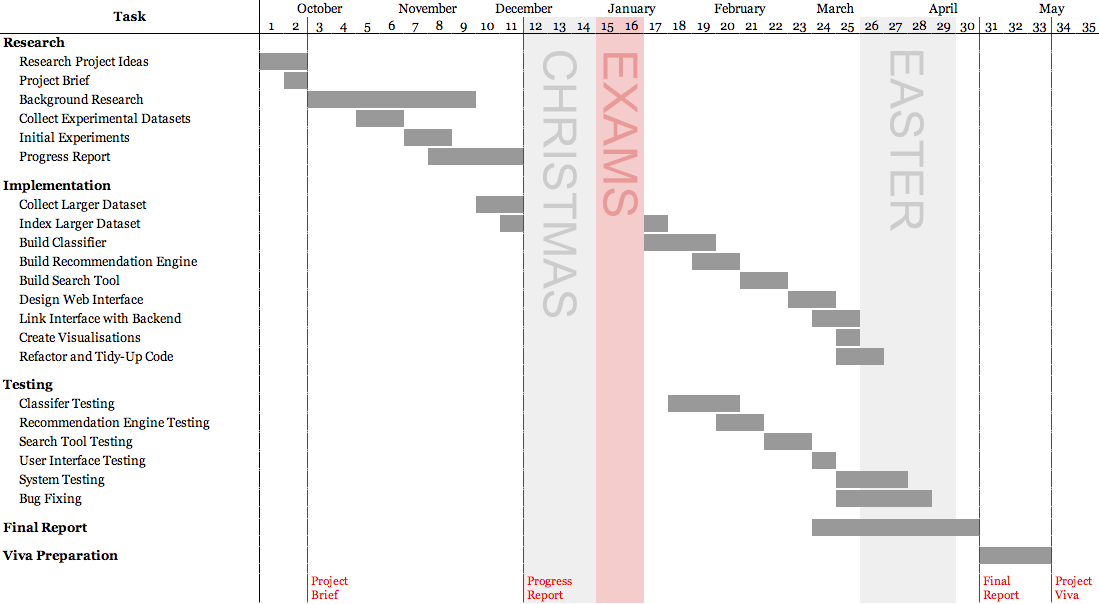
\includegraphics[height=0.85\textwidth]{gantt.png}
    \end{figure}
\end{landscape}

\setcounter{secnumdepth}{0}
\section{References}
{\footnotesize \printbibliography[heading=none]}

\end{document}
